\documentclass[../basicOrbitalDynamics.tex]{subfiles}
\graphicspath{{\subfix{../images/}}}
\begin{document}

%TODO: HEADER

\bigskip\bigskip
\subsection{Geosynchronous Orbits (WIP)}\label{Geosynchronous Orbits}

%TODO

\bigskip\bigskip
\subsection{Lagrange Points (WIP)}\label{Lagrange Points}

Up to this point, trajectories have all assumed a single gravitational influence. Section \ref{Patched Conics} described how to use this approximation to generate trajectories between multiple bodies. However, by taking into account multiple gravitational attractors, otherwise impossible trajectories can be generated.

To motivate this subject, we will consider a lunar signal relay spacecraft. An orbital engineer wants to find an orbit for a satellite that will keep it at the same spot between Earth and the moon at all times, with the purpose of relaying signals from Earth-based communications networks to moon-orbiting satellites. For the sake of this example, the moon's orbit about Earth can be approximated (within reason) to be perfectly circular. Because the satellite is between Earth and the moon, $0<\st{a}{sat}<\st{a}{moon}$.In order for this spacecraft to achieve the desired orbit, its orbital period must match that of the moon. Recall from Eqaution \eqref{Period Geometric} that the period of an orbit is

$$T=\sqrt{\frac{4\pi^2 a}{\mu}}$$
Using this equation, it is clearly impossible for the satellite and the moon to have the same period, as their semi-major axes are different. Neglecting any other gravitational influences, a satellite between Earth and the moon would have to move faster than the moon in order to remain in a circular orbit, and would also have to a further distance to go (a larger orbit means a larger circumference). However, if some force can pull the satellite away from Earth, it will be able to orbit slower at the same altitude. The moon can provide such a force on the satellite. If instead the satellite wants to keep the moon between it and Earth at all times, it would require a downward force, which, if the moon is between it and Earth, the moon can provide. Because of the moon's gravitational influence on the satellite, most orbits at lunar orbital altitude would be unstable. However, the gravitational influence of the moon makes three of them stable. These points at which the satellite can orbit are called Lagrange points, and they exist in any two-body system. Lagrange points will be generalized to be between any two masses $M_1$ and $M_2$, some distance $R$ apart.

The most interesting Lagrange points are the ones that lie on either side of the smaller body along the line extending between both. These are known as L1 (in the Earth-moon system, between Earth and the moon), and L2 (on the opposite side of the moon as Earth). The Lagrange points can be found analytically. To make calculations easier, it will be assumed that $M_2<<M_1$, so that $M_2$ orbits about $M_1$'s center of mass, with $M_1$'s inertial acceleration being negligible.

\begin{figure}[H]
    \centering
    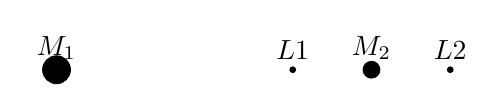
\begin{tikzpicture}[>=latex]
        \filldraw[] (0,0) circle (5pt) node[above] {$M_1$};
        \filldraw[] (4,0) circle (3pt) node[above] {$M_2$};
        \filldraw[] (3,0) circle (1pt) node[above] {$L1$};
        \filldraw[] (5,0) circle (1pt) node[above] {$L2$};
%        \node[circle, fill=white, draw=gray] at (0,0) {$M_1$};
%        \node[circle, fill=white, draw=gray] at (3,0) {$M_2$};

    \end{tikzpicture}
    \caption{Locations of L1 and L2 in a system with two masses}\label{fig:Lagrange Points}
\end{figure}

\subsubsection{L1 Lagrange Point}

We will begin with Newton's second law

$$\st{\vv{F}}{net}=m\vv{a}$$

To use the Transport Theorem (see Section \ref{Sec:Motion}) to find the required inertial acceleration $\vv{a}$ in the above equation, the angular velocity $\omega$ of the smaller body (in the Earth-moon system, this would be the moon) must be found. $\omega$ can be expressed as the velocity divided by the radius. $V$ denotes the velocity of $M_2$ about $M_1$ at their distance $R$ apart. Recall circular velocity from Equation \eqref{Circular Velocity}.

\begin{align*}
    \omega&=\frac{V}{R}\\
    \omega&=\frac{\sqrt{\mu/R}}{R}\\
    \omega&=\sqrt{\frac{\mu}{R^3}}\\
\end{align*}

With this calculated, the required polar acceleration can be calculated. The satellite's orbital radius about $M_1$ is $r$

\begin{align*}
    \vv{v}^{r\theta{}n}&=\frac{d^{xyz}}{dt}{\vv{r}^{r\theta{}n}}+\prescript{xyz}{}{\omega}^{r\theta{}n}\times{}\vv{r}^{r\theta{}n}\\
    &=\frac{d^{xyz}}{dt}{r\hat{u}_r}+\sqrt{\frac{\mu}{R^3}}\hat{u}_n\times r\hat{u}_r\\
    &=\sqrt{\frac{\mu r^2}{R^3}}\hat{r}_\theta\\
\end{align*}

This can be differentiated to find acceleration

\begin{align*}
    \vv{a}^{r\theta{}n}&=\frac{d^{xyz}}{dt}{\vv{v}^{r\theta{}n}}+\prescript{xyz}{}{\omega}^{r\theta{}n}\times{}\vv{v}^{r\theta{}n}\\
    &=\frac{d^{xyz}}{dt}\sqrt{\frac{\mu r^2}{R^3}}\hat{r}_\theta+\sqrt{\frac{\mu}{R^3}}\hat{u}_n\times \sqrt{\frac{\mu r^2}{R^3}}\hat{r}_\theta\\
    &=-\sqrt{\frac{\mu}{R^3}}\sqrt{\frac{\mu r^2}{R^3}}\hat{r}_n\\
    &=-\sqrt{\frac{\mu^2 r^2}{R^6}}\hat{r}_n\\
    &=-\frac{\mu r}{R^3}\hat{r}_n\\
\end{align*}

The polar acceleration on the satellite for it to maintain its orbit is

$$\st{\vv{a}}{polar}=-\frac{\mu r}{R^3}\hat{r}_n$$

From Equation \eqref{Gravity} (and Newton's second law), the polar acceleration of gravity in the radial direction is
$$a_g=\frac{GM}{d^2}$$

Where $\mu$ has been replaced with $GM$, and $d$ is the distance to the body. The direction of the acceleration is toward the attracting body. At $L1$, $M_2$ will provide radially outward acceleration while $M_1$ will provide radially inward acceleration. An equation can now be set up to find $\alpha_{r1}$, the ratio of distance between $L1$ and $M_1$ and that of $M_1$ and $M_2$ (in other words, $\alpha_{L1}=r/R$).
\begin{align*}
    a_1+a_2&=\st{a}{net}\\
    -\frac{GM_1}{(R\alpha_{L1})^2}+\frac{GM_2}{(R(1-\alpha_{L1}))^2} &= -\frac{\mu_1 r}{R^3}\\
    -\frac{GM_1}{(R\alpha_{L1})^2}+\frac{GM_2}{(R(1-\alpha_{L1}))^2} &= -\frac{GM_1 R\alpha_{L1}}{R^3}\\
    -\frac{M_1}{\alpha_{L1}^2}+\frac{M_2}{(1-\alpha_{L1})^2} &= -M_1\alpha_{L1}\\
    -M_1(1-\alpha_{L1})^2+M_2\alpha_{L1}^2 &= -M_1\alpha_{L1}^3(1-\alpha_{L1})^2\\
    M_1\alpha_{L1}^3(1-\alpha_{L1})^2-M_1(1-\alpha_{L1})^2+M_2\alpha_{L1}^2 &= 0\\
    M_1(\alpha_{L1}^3-2\alpha_{L1}^4+\alpha_{L1}^5)+M_1(-1+2\alpha_{L1}-\alpha_{L1}^2)+M_2\alpha_{L1}^2 &= 0\\
    M_1\alpha_{L1}^5-2M_1\alpha_{L1}^4+M_1\alpha_{L1}^3+(M_2-M_1)\alpha_{L1}^2+2M_1\alpha_{L1}-M_1&= 0\\
\end{align*}

This is not solveable analytically, but it can be solved numerically. The entire expression will be divided by $M_1$ to make it simpler.
\begin{equation}\label{L1 Equation}
    \left(\frac{r_{L1}}{R}\right)^5-2\left(\frac{r_{L1}}{R}\right)^4+M_1\left(\frac{r_{L1}}{R}\right)^3+\left(\frac{M_2}{M_1}-1\right)\left(\frac{r_{L1}}{R}\right)^2+2\left(\frac{r_{L1}}{R}\right)-1= 0
\end{equation}

\bigskip\bigskip
\subsection{Time over the Horizon (WIP)}

% TODO https://www.desmos.com/calculator/kyyuqzonoy, add rotation of the planet

\bigskip\bigskip
\subsection{Conclusion}

\end{document}